\section{My research interests}

\subsection{Stochastic differential equations}

\subsubsection*{Simulation schemes for path-dependent options\footnote{\fullcite{gobet2000weak}}}

We are interested in a path-dependent payoff on an asset with diffusion $(X_t)_{0\leq t \leq T}$.
In particular, we kill the diffusion when it leaves the open set $D$.
\newline With $\tau \coloneqq \inf\{t > 0 : X_t \notin D\}$, this leads to the computation of $\mathbb{E}\left[\mathbbm{1}_{T < \tau} f(X_T)\right].$

\begin{proposition}
    Price of a double no-touch option with lower and upper barriers $S_{min}$, $S_{max}$:


$$V(S,t) = 2\pi \left(\dfrac{S}{S_{min}}\right)^{\alpha} e^{\beta(T-t)} \sum_{n=1}^{\infty} n \left[\dfrac{(1 - (-1)^{m}e^{-\alpha H})}{\alpha^2 H^2 + n^2 \pi^2} \right] \exp \left(-\frac{1}{2}\sigma^2 \dfrac{n^2 \pi^2}{H^2} t \right) \sin \left(\dfrac{n\pi}{H} \ln \frac{S}{S_{min}} \right).$$

with $H=\ln(S_{max}/S_{min})$, $\alpha = -\Tilde{r}/\sigma^2$ and $\beta = -\Tilde{r}/ 2\sigma^2 - r$, $\Tilde{r} = r - \frac{1}{2}\sigma^2$.
\end{proposition}

\begin{proof}
    See \ref{appendix:a}
\end{proof}

\begin{figure}[H]
    \centering
    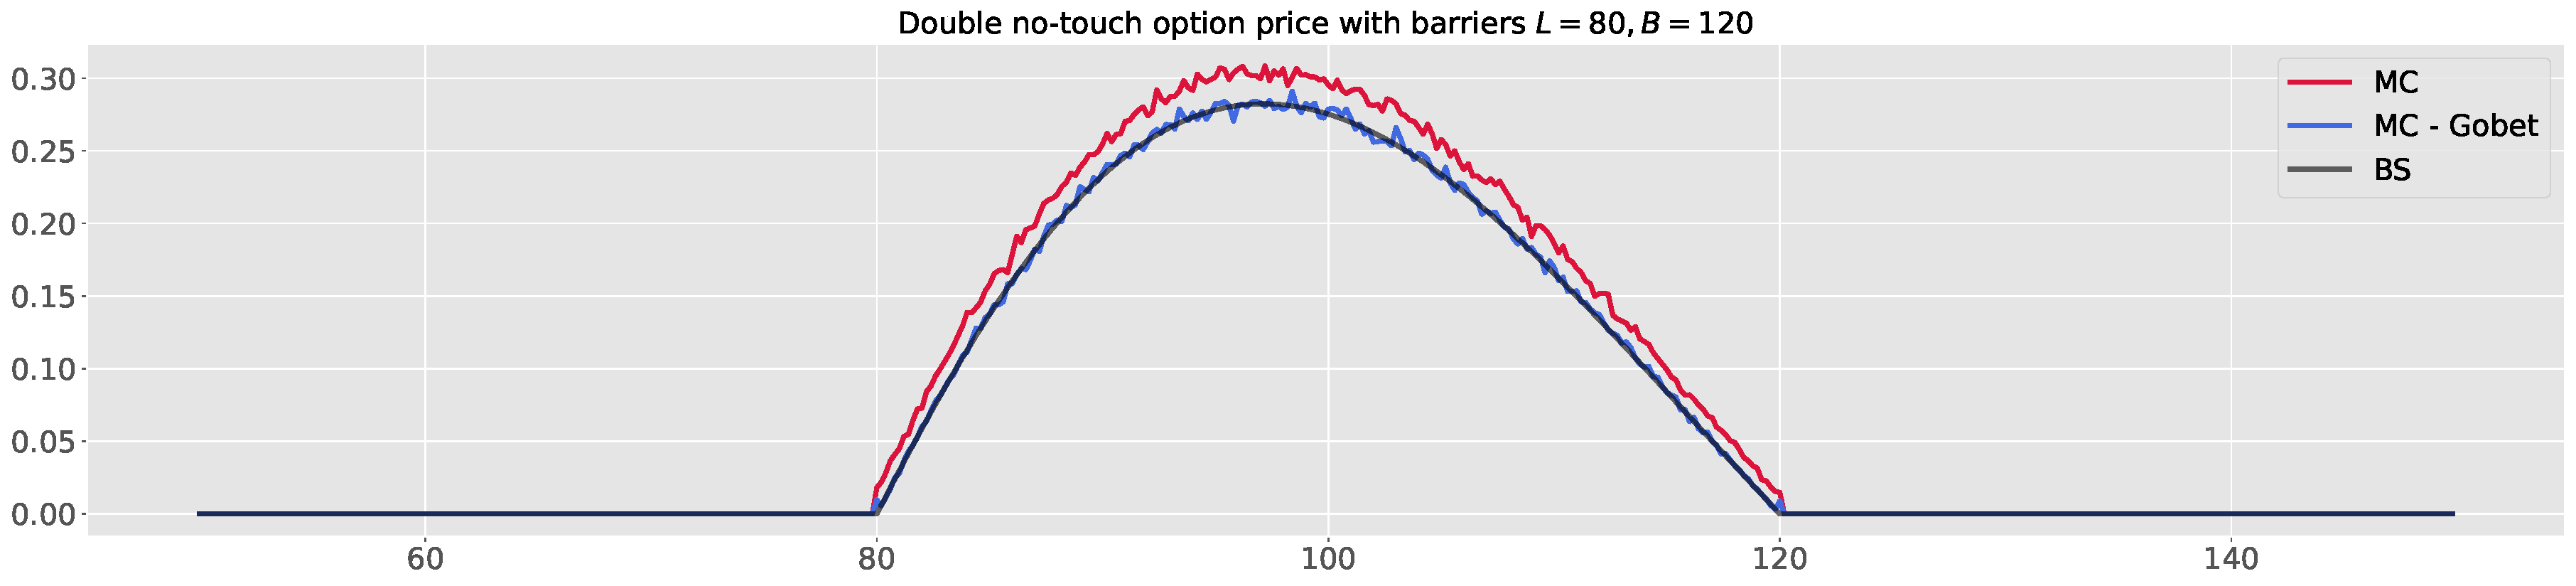
\includegraphics[width=1\linewidth]{img/dnt_mc.pdf}
    \caption{Evolution of the double no-touch option that pays $\$1$ against $S_0$}
    \label{fig:doublenotouchmc}
\end{figure}

\subsection{Deep learning}

\cite{gobet2000weak}

\subsubsection*{Generating synthetic data\footnote{\fullcite{kondratyev2019market}}}

Monte Carlo risk engines based on historical events may lead to an overfitting in the backtesting process. Being able to generate unseen yet but coherent market scenarios can be crucial from a risk-management perspective.
In mathematical terms, generating realistic market scenarios is "sampling from the joint distribution of risk factors". A simple \textbf{parametric} approach to this problem would be calibrating a normal law to the distribution of log-returns and sampling from it. This empirical distribution exhibiting -- among other particularties -- skewness and kurtosis \cite{cont2001empirical}, it is often a poor approximation of reality.\newline
Alternative \textbf{non-parametric} approaches can be found in Generative Adversarial Network (GAN) \cite{goodfellow2014generative}, where the target distribution is directly learned from the data without the need for assumptions about the form of it. With this framework though, we are already entering the realm of neural networks.


\begin{figure}[H]
    \centering
    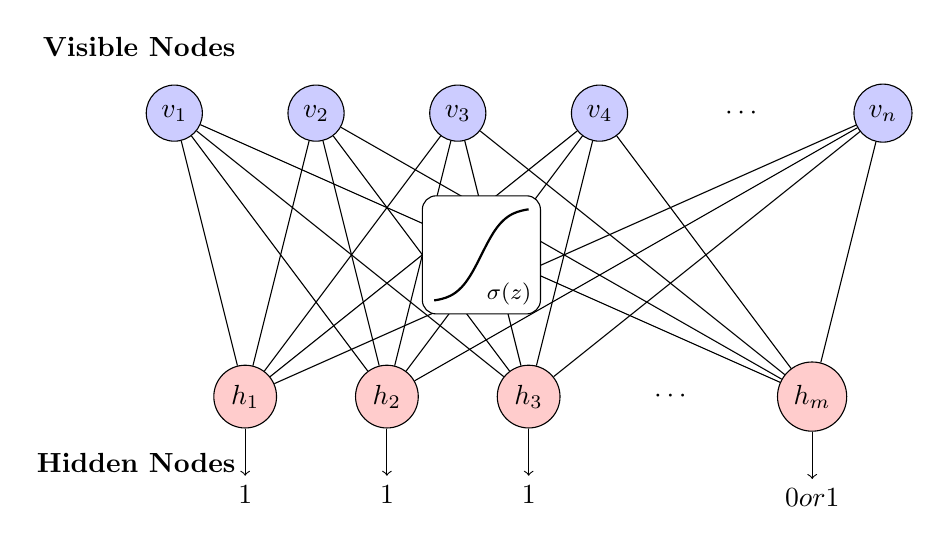
\begin{tikzpicture}[scale=1.2]

    % Parameters
    \def\nbhid{3}
    \def\nbvis{4} % Change to desired number of visible nodes
    
    % Calculate center position for visible nodes
    \pgfmathsetmacro\centerVis{(\nbvis-1)/2}
    % Calculate center position for hidden nodes
    \pgfmathsetmacro\centerHid{(\nbhid-1)/2}
    
    % Define hidden nodes
    \foreach \y in {1,2,...,\nbhid}
        \node[draw, circle, fill=red!20] (h\y) at (\y*1.5-\centerHid*1.5,0) {$h_\y$};
    
    % Add dots for hidden nodes
    \node[draw=none, fill=none] (hdots1) at (\nbhid*1.5+1.5-\centerHid*1.5,0) {$\cdots$};
    \node[draw, circle, fill=red!20] (hm) at (\nbhid*1.5+3-\centerHid*1.5,0) {$h_m$};

    % Define visible nodes
    \foreach \x in {1,2,...,\nbvis}
        \node[draw, circle, fill=blue!20] (v\x) at (\x*1.5-\centerVis*1.5,3) {$v_\x$};
    
    % Add dots for visible nodes
    \node[draw=none, fill=none] (vdots1) at (\nbvis*1.5+1.5-\centerVis*1.5,3) {$\cdots$};
    \node[draw, circle, fill=blue!20] (vn) at (\nbvis*1.5+3-\centerVis*1.5,3) {$v_n$};
    
    % Connect visible nodes to hidden nodes
    \foreach \x in {1,2,...,\nbvis}
        \foreach \y in {1,2,...,\nbhid}
            \draw (v\x) -- (h\y);
    
    % Connect vn to hidden nodes and hm
    \foreach \y in {1,2,...,\nbhid}
        \draw (vn) -- (h\y);
    \foreach \x in {1,2,...,\nbvis}
        \draw (hm) -- (v\x);
    \draw (vn) -- (hm);
    
    % Add arrows indicating random firing
    \foreach \y in {1,2,...,\nbhid} {
        \pgfmathsetmacro{\rand}{random(0,1)}
        \ifnum\rand=0
            \def\lbl{0}
        \else
            \def\lbl{1}
        \fi
        \draw[->] (h\y.south) -- ++(0,-0.5) node[below] {$\lbl$};
    }

    \draw[->] (hm.south) -- ++(0,-0.5) node[below] {$0 \text{ or } 1$};

    % Activation
    \node[draw, rectangle, fill=white, minimum width=1.5cm, minimum height=1.5cm, rounded corners=5pt] (sigmoid) at (\centerVis+1,1.5) {};
    \draw[thick, domain=-0.5:0.5, smooth, variable=\x, black]  plot ({\x+\centerVis+1}, {1+ 1/(1+exp(-\x*8))});
    \node[black, font=\footnotesize, anchor=south east] at (sigmoid.south east) {$\sigma(z)$};


    
    % Add labels
    \node[above left, font=\bfseries] at (0,3.5) {Visible Nodes};
    \node[below left, font=\bfseries] at (0,-0.5) {Hidden Nodes};

\end{tikzpicture}
    \caption{Bernoulli Restricted Boltzmann Machine (RBM) bipartite graph}
    \label{fig:rbm}
\end{figure}


